% TBP-double-Ag100
\paragraph{Unit cell}
When adsorbed on a square (100) silver surface, the molecules interestingly arrange in a trihexagonal tiling (see figure \ref{fig:two-leg-trans-ag100-motif}). The molecules at the perimeter of this island is nicely distinguishable and continuing their regular pattern to the center of the island results in an accurate description of the assembly. The unit cell is determined to be $\underline{\qquad \qquad}$ and the hexagonal unit cell is shown in \autoref{fig:two-leg-trans-ag100-unit-cell}, bearing three molecules.\footnote{Similar open porous network can be created, e.g. cyano functionalized triarylamines on Au(111) \cite{gottardi_cyano-functionalized_2014}.}

\paragraph{Molecular orientation}
The molecules are arranged so that each molecule has one of its di-tert-butyl-groups in one hexagonal pores and the other in the neighboring one. Each pore is made up of six molecules arranged on a hexagon with $\underline{\qquad \qquad}$ long edges. Each vertex is occupied by a single molecule, neighboring molecules on the hexagon are rotated by \SI{60}{\degree}. The pores are created by free space where the di-tert-butyl-groups point towards each other. The nitro-phenyl groups point towards the intermediate space where smaller triangular openings are formed. At their edges the nitro-phenyl groups connect to the neighboring di-tert-butyl groups.

Considering a former orientation calibration on Ag(100) where the direction of the dense packed crystal direction was determined, the orientation with regard to the substrate is given as white lines in \autoref{fig:two-leg-trans-ag100-unit-cell}: The long and short axis of the unit cell (marked as green cross in \subref{fig:two-leg-trans-ag100-unit-cell}) is almost collinear, just differing by less than \SI{10}{\degree}. Since the calibration was done with another preparation the angle calibration may not be \SI{100}{\percent} accurate because the sample was moved in the meantime. That may result in an little angle uncertainty. Please see  \autoref{F160429-185245-R-model-2-crystal-orientation.png} in \fullref{appendix:TBP} for a detailed image.

\paragraph{Contrast within single molecule}
A closer look to the geometries in high resolution STM data gives clue to the rotation of the di-tert-butyl-groups and is visualized in \autoref{fig:two-leg-trans-ag100-single-molecule}. Focusing on the STM contrast of a single molecule, one can see that it is dominated by the di-tert-butyl-groups on both sides of the molecule. These look like small triangles in the STM with a single brighter protrusion enclosed by the footprint. The bright protrusion is never on the same side of the triangular footprint thus the di-tert-butyl-groups are believed to be rotated in two different directions - lifting opposite parts of the functional group.
\begin{figure}[]
	\centering
	\subfigure[STM topography of several islands grown next to a step edge. Areas with trihexagonal tiling as well as some domain boundaries are visible.]{
		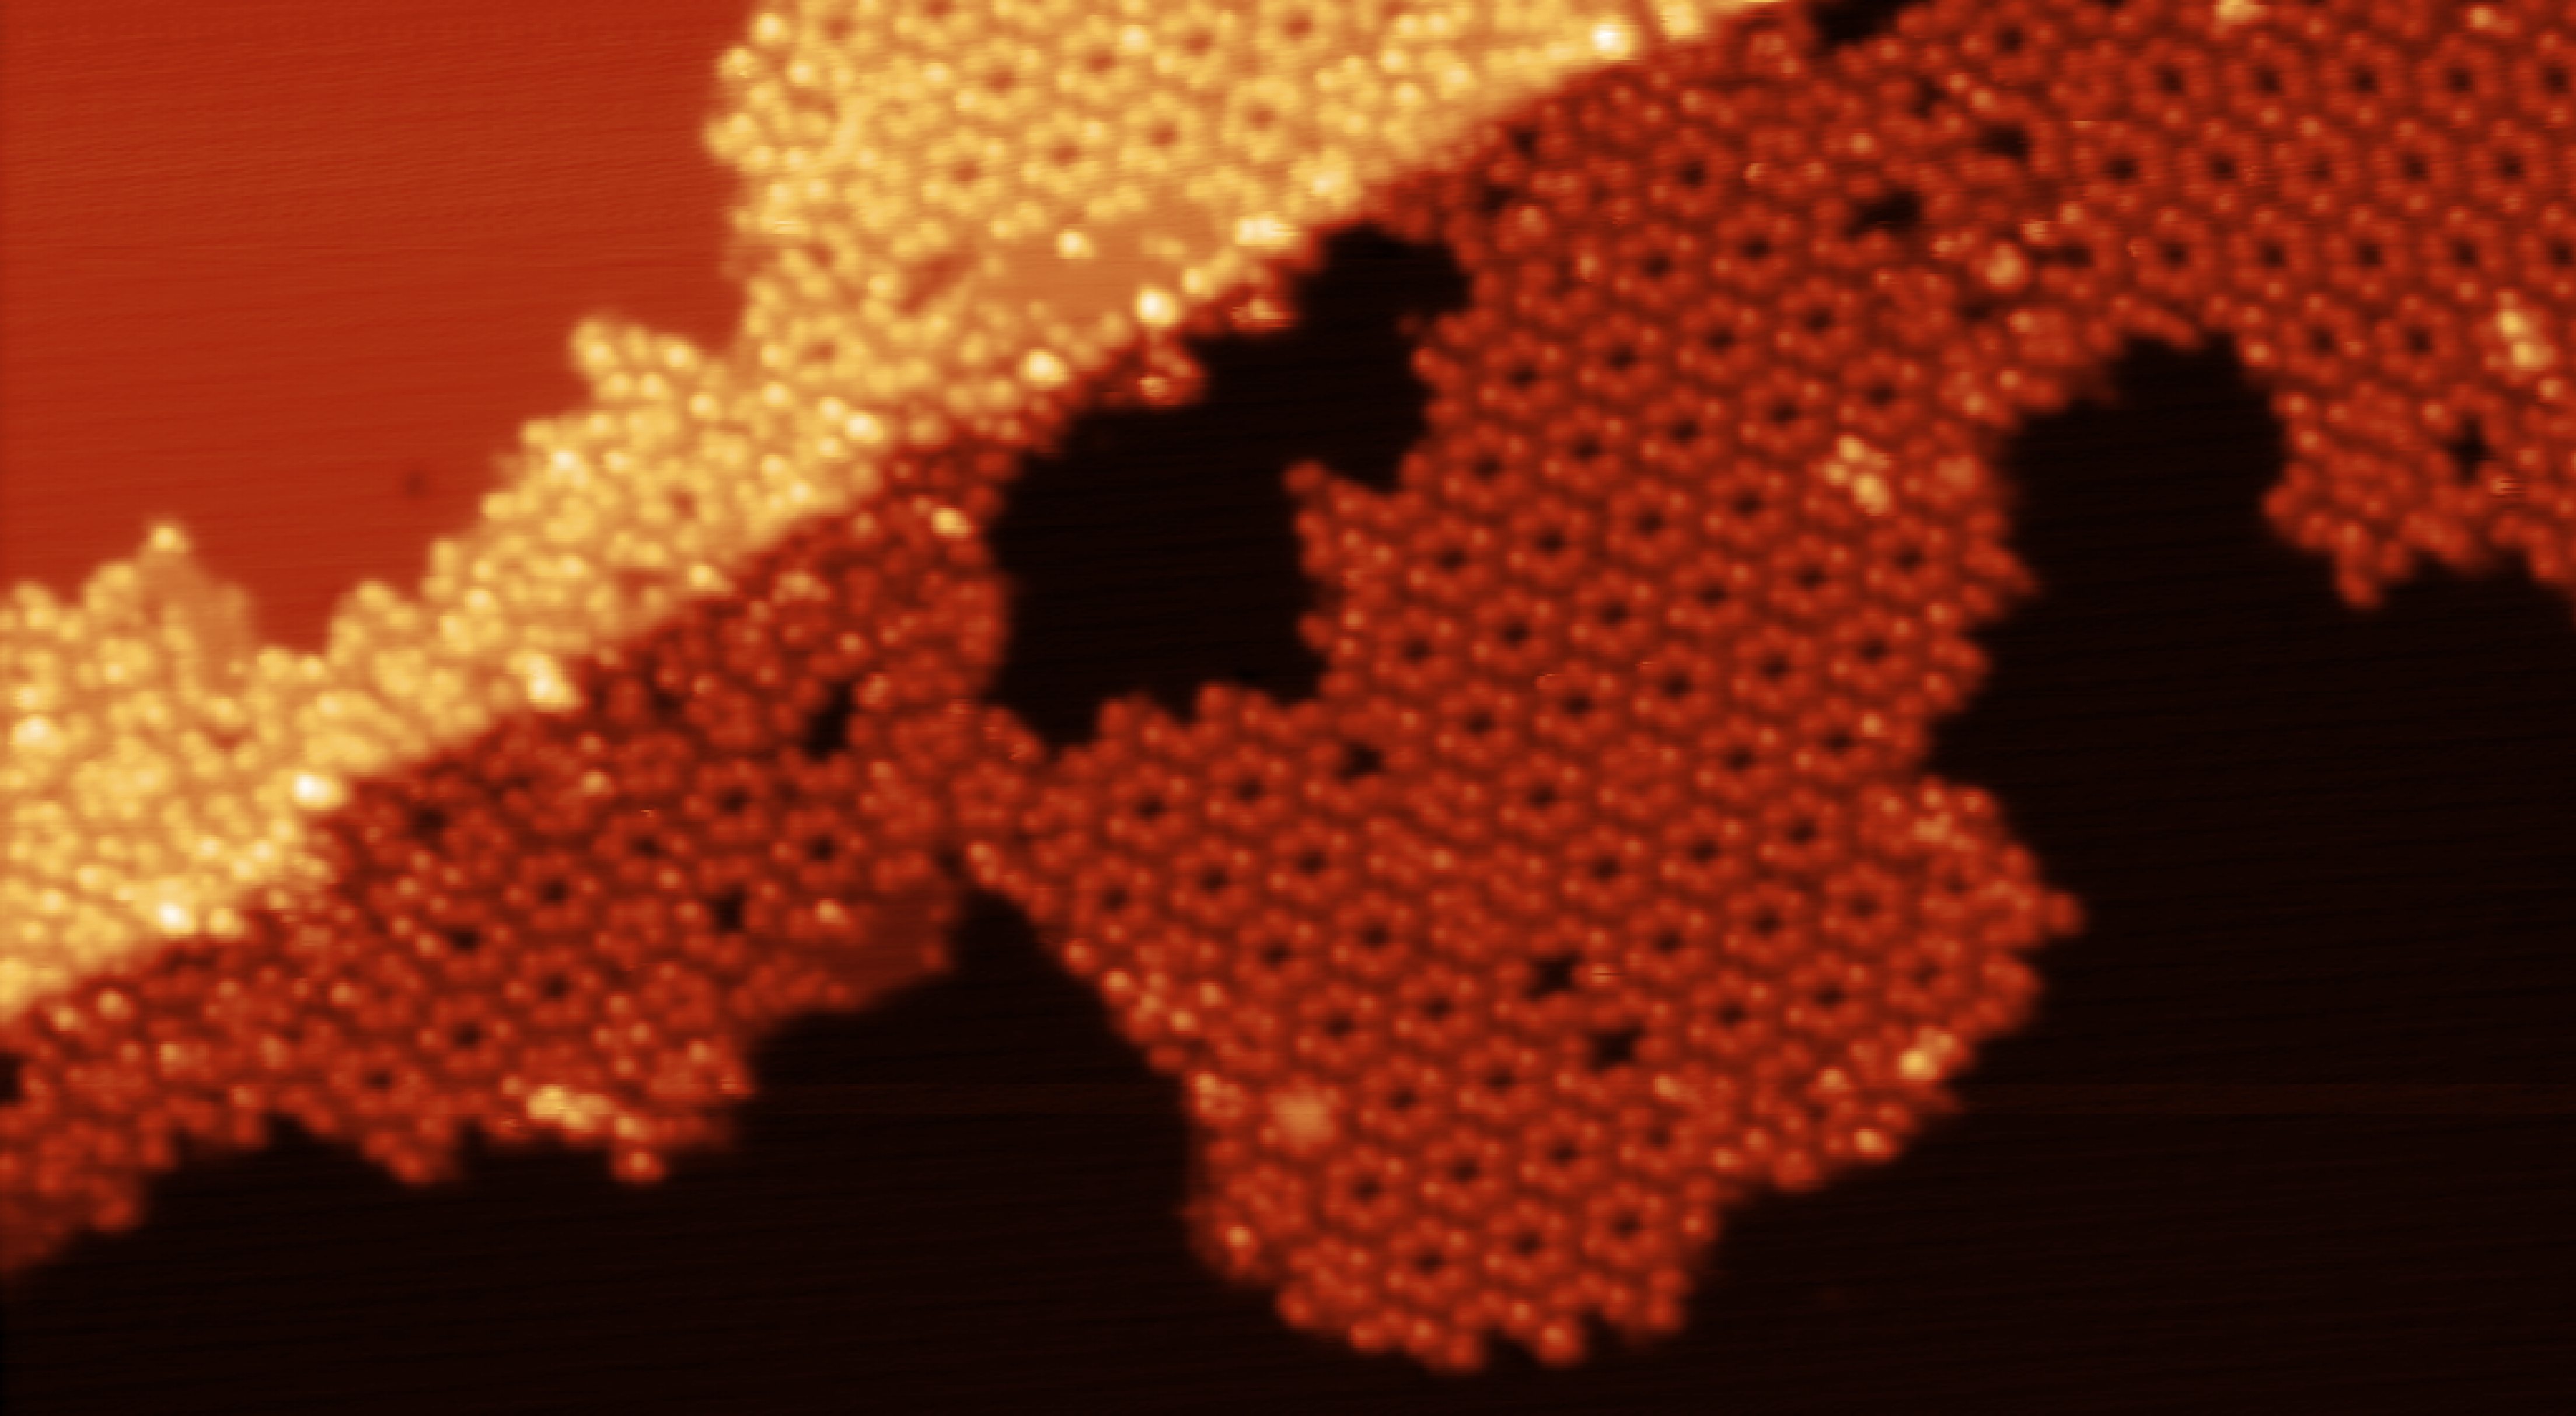
\includegraphics[width=\textwidth]{./images/F160429-172019}
		\label{fig:two-leg-trans-ag100-overview}
	} %COARSE MODE!
	\subfigure[Hexygonal unit cell with overlaid molecular models.]{
		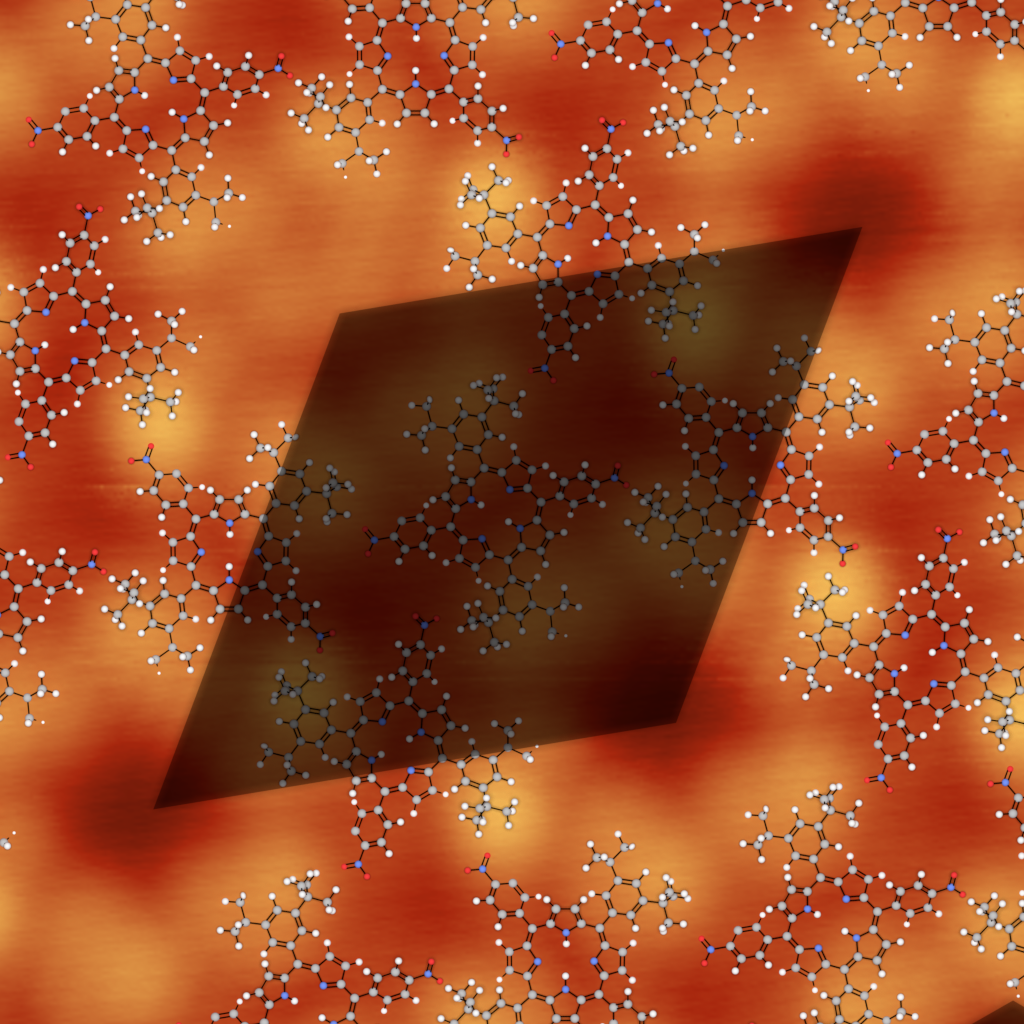
\includegraphics[width=0.3\textwidth]{./images/F160429-185245-R-model}
		\label{fig:two-leg-trans-ag100-unit-cell}
	} \quad %COARSE MODE!
	\subfigure[Enlarged view on the molecules rotated di-tert-butyl-group and highest elements enclosed by brighter circles..]{
		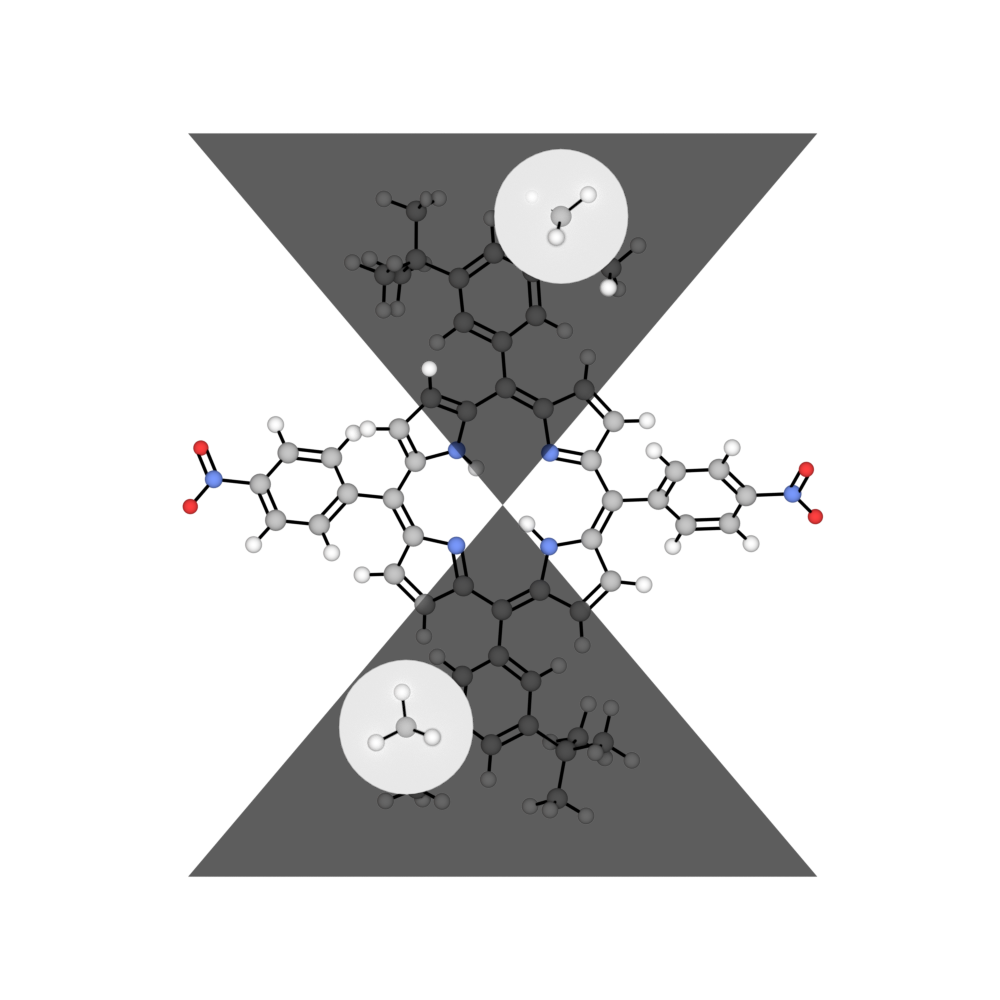
\includegraphics[width=0.3\textwidth]{./images/F160429-185245-R-single-molecule}
		\label{fig:two-leg-trans-ag100-single-molecule}
	} %COARSE MODE!
	\caption{Trans-TBP adsorped on Ag(100) at room temperature. \subref{fig:two-leg-trans-ag100-overview} shows a large overview of the assembled molecules. The unit cell constituents are enlarged in \subref{fig:two-leg-trans-ag100-unit-cell} where parts of \subref{fig:two-leg-trans-ag100-overview} are shown with molecular models overlaid. \subref{fig:two-leg-trans-ag100-single-molecule} shows a single molecule crossing a horizontal plain to emphasize high lying part in the molecule that are marked with white circles and will appear brighter in STM. All images recorded with \SI{437}{\milli\volt}, \SI{0.1}{\nano\ampere}, color scale \SIrange{0}{650}{\pico\meter}
	}
	\label{fig:two-leg-trans-ag100-motif}
\end{figure}

\paragraph{Domain boundaries}
The observed domain boundaries are imaged in \autoref{fig:two-leg-trans-ag100-domain-boundary}. On both sides the regular tiling is proceeded, but both are shifted with respect to each other by $\underline{\qquad \qquad}$. This offset results in the wrong alignment of molecules from one  domain with respect to the other domain and a discontinued growth. The resulting free area at the domain boundary is occupied by molecules from one domain that bear the wrong orientation the proceed the growth of the second domain and vice versa. This can be nicely seen in 		\autoref{fig:two-leg-trans-ag100-domain-molecular-model}, where the misalignment of one domain (left) with respect to the other (right) causes two cavities to open up between the two (lower image part). While these two are unoccupied and reveal the substrate, another type of cavity can be formed directly seen on top of the two aforementioned. Here the cavity is filled with a single molecule so that both di-tert-butyl groups interlock with the open cavity. Please note that some is the assembly pores are filled, too. Here the space of the pore prohibits a complete molecule to fit in, the observed adsorbates in the pores are most likely molecular fragments like tert-butyl-groups that were incorporated by the assembly during the island growth.

\begin{figure}[]
	\centering
	\subfigure[Domain boundary]{
		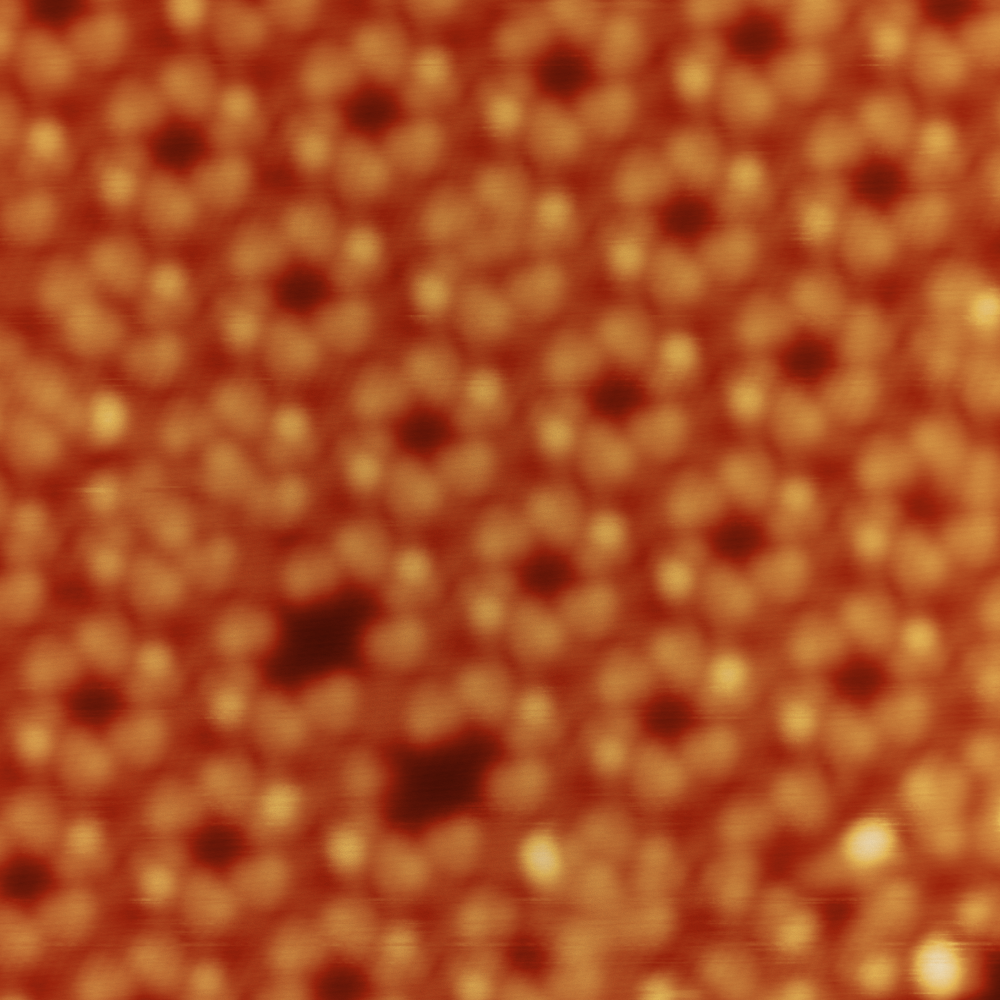
\includegraphics[width=0.35\textwidth]{./images/F160429-185245-R--2}
		\label{fig:two-leg-trans-ag100-domain-overview}
	} %COARSE MODE!
	\subfigure[Model representation of domain boundary]{
		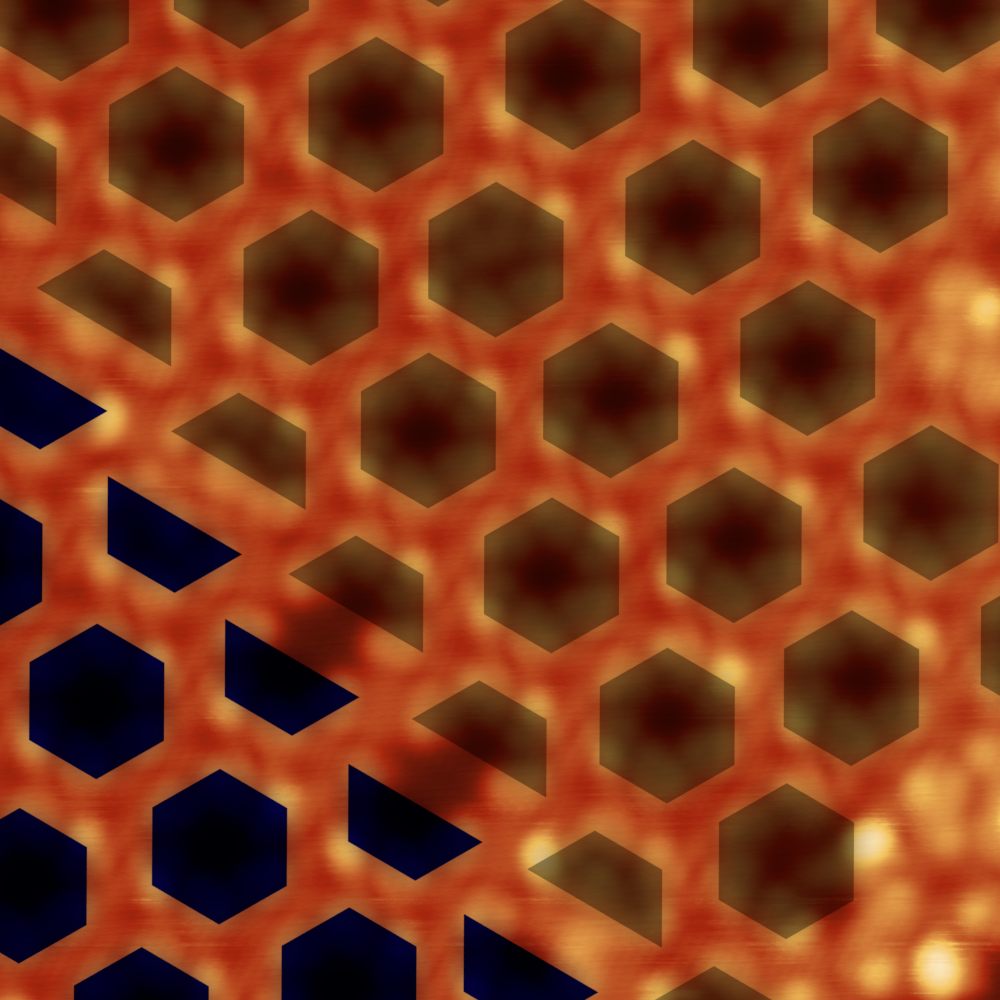
\includegraphics[width=0.35\textwidth]{./images/F160429-185245-R--2-model}
		\label{fig:two-leg-trans-ag100-domain-model}
	} %COARSE MODE!
	\subfigure[Molecular model of domain boundary, overlaid with two unit cells]{
		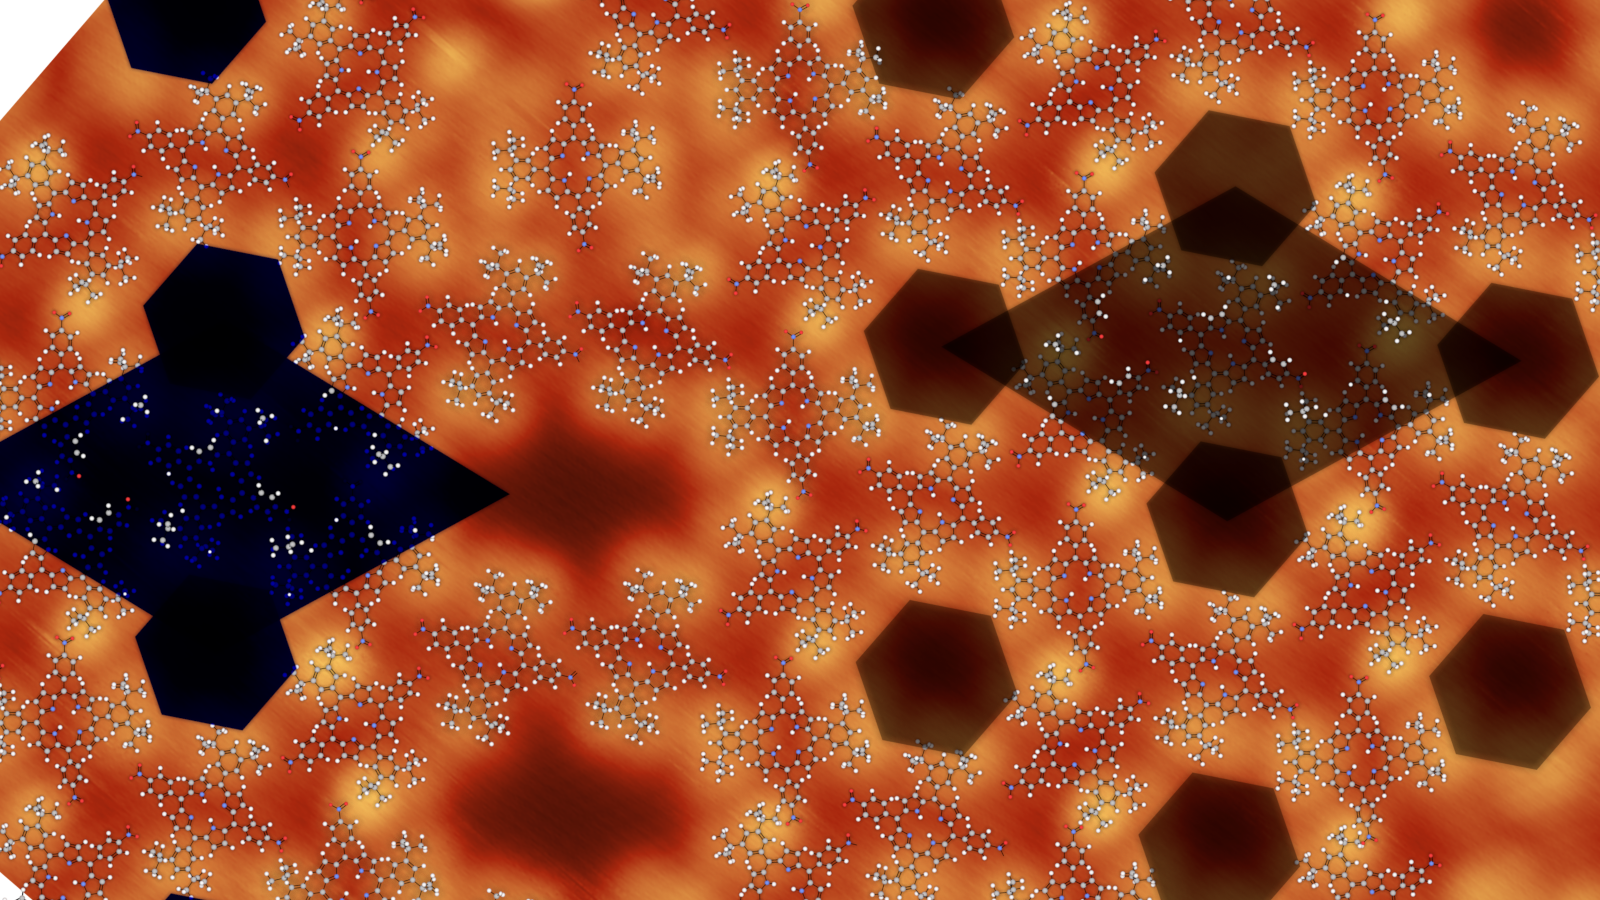
\includegraphics[width=0.7\textwidth]{./images/F160429-185245-R--domain-overview}
		\label{fig:two-leg-trans-ag100-domain-molecular-model}
	} \quad %COARSE MODE!
	\caption{Domain boundary of trans-TBP adsorbed on Ag(100) at RT. \subref{fig:two-leg-trans-ag100-domain-overview} shows an overview of the domain boundary together with its model representation in \subref{fig:two-leg-trans-ag100-domain-model}. The assembly close by is modeled in \subref{fig:two-leg-trans-ag100-domain-molecular-model} where parts of \subref{fig:two-leg-trans-ag100-domain-overview} are shown and molecular models overlaid. All images recorded with \SI{1.3}{\volt}, \SI{0.1}{\nano\ampere}, color scale \SIrange{0}{650}{\pico\meter}
	}
	\label{fig:two-leg-trans-ag100-domain-boundary}
\end{figure}